\chapter{Multivariantna statistika}

Povezanost med spremenljivkama ne pomeni nujno, da med njima obstaja vzročna povezava. Spremenljivke so lahko povezane tudi navidezno, pri čemer se pojasni uvedba tretje spremenljivke (npr. poletni čas pojasni povezavo med napadi morskih psov in prodajo sladoleda).

\section{Multipla regresijska analiza (linearna)}

Multipla regresijska analiza je metoda za preučevanje razmerja med odvisno spremenljivko in dvema ali več neodvisnimi spremenljivkami. Namen je napovedovanje vrednosti odvisne spremenljivke z nizom neodvisnih spremenljivk.

Regresijski model je podan kot:
\[Y = \beta_0 + \beta_1 X_1 + \ldots + \beta_k X_k,\]
kjer je:
\begin{itemize}
    \item $Y$ odvisna spremenljivka,
    \item $X_1, \ldots, X_k$ neodvisne spremenljivke,
    \item $\beta_0$ presečišče (intercept),
    \item $\beta_1, \ldots, \beta_k$ regresijski koeficienti, ki kažejo na spremembo v $Y$ pri enotni spremembi $X_i$,
    \item $\epsilon$ napaka modela.
\end{itemize}

\paragraph{Izračun koeficientov $\beta_i$}
Regresijski koeficienti $\beta_i$ se izračunajo z metodo najmanjših kvadratov, ki minimizira vsoto kvadratov odstopanj predvidenih vrednosti od dejanskih vrednosti:
\[
\hat{\beta} = (X'X)^{-1}X'Y
\]
kjer je $X$ matrica neodvisnih spremenljivk, $Y$ pa vektor odvisne spremenljivke.

\paragraph{Koeficient determinacije $R^2$}
Delež variabilnosti, ki ga model pojasni, je izražen z $R^2$, ki ga izračunamo kot:
\[R^2 = 1 - \frac{\sum_{i=1}^{n} (Y_i - \hat{Y}_i)^2}{\sum_{i=1}^{n} (Y_i - \bar{Y})^2},\]
kjer:
\begin{itemize}
    \item $\hat{Y}_i$ so napovedane vrednosti odvisne spremenljivke,
    \item $Y_i$ so dejanske vrednosti odvisne spremenljivke,
    \item $\bar{Y}$ je povprečje odvisne spremenljivke.
\end{itemize}

$R^2$ meri delež skupne variabilnosti v odvisni spremenljivki, ki jo je mogoče pojasniti z regresijskim modelom. Vrednost $R^2$ se giblje med 0 in 1, pri čemer 1 pomeni popolno prileganje modela podatkom.

Pomembno je, da velikost vzorca zadostuje za stabilnost ocenjenih koeficientov. Priporočeno je, da je velikost vzorca vsaj 10-krat večja od števila neodvisnih spremenljivk.

\paragraph{Predpostavke multiple linearne regresije}
\begin{itemize}
    \item \textbf{Neodvisnost}: Opazovanja so neodvisna.
    \item \textbf{Normalnost}: Napake v regresijskem modelu so normalno porazdeljene.
    \item \textbf{Homoskedastičnost}: Variabilnost napak je konstantna pri vseh nivojih neodvisnih spremenljivk.
    \item \textbf{Linearnost}: Obstaja linearna povezava med odvisno in neodvisnimi spremenljivkami.
\end{itemize}

\begin{figure}[h]
    \centering
    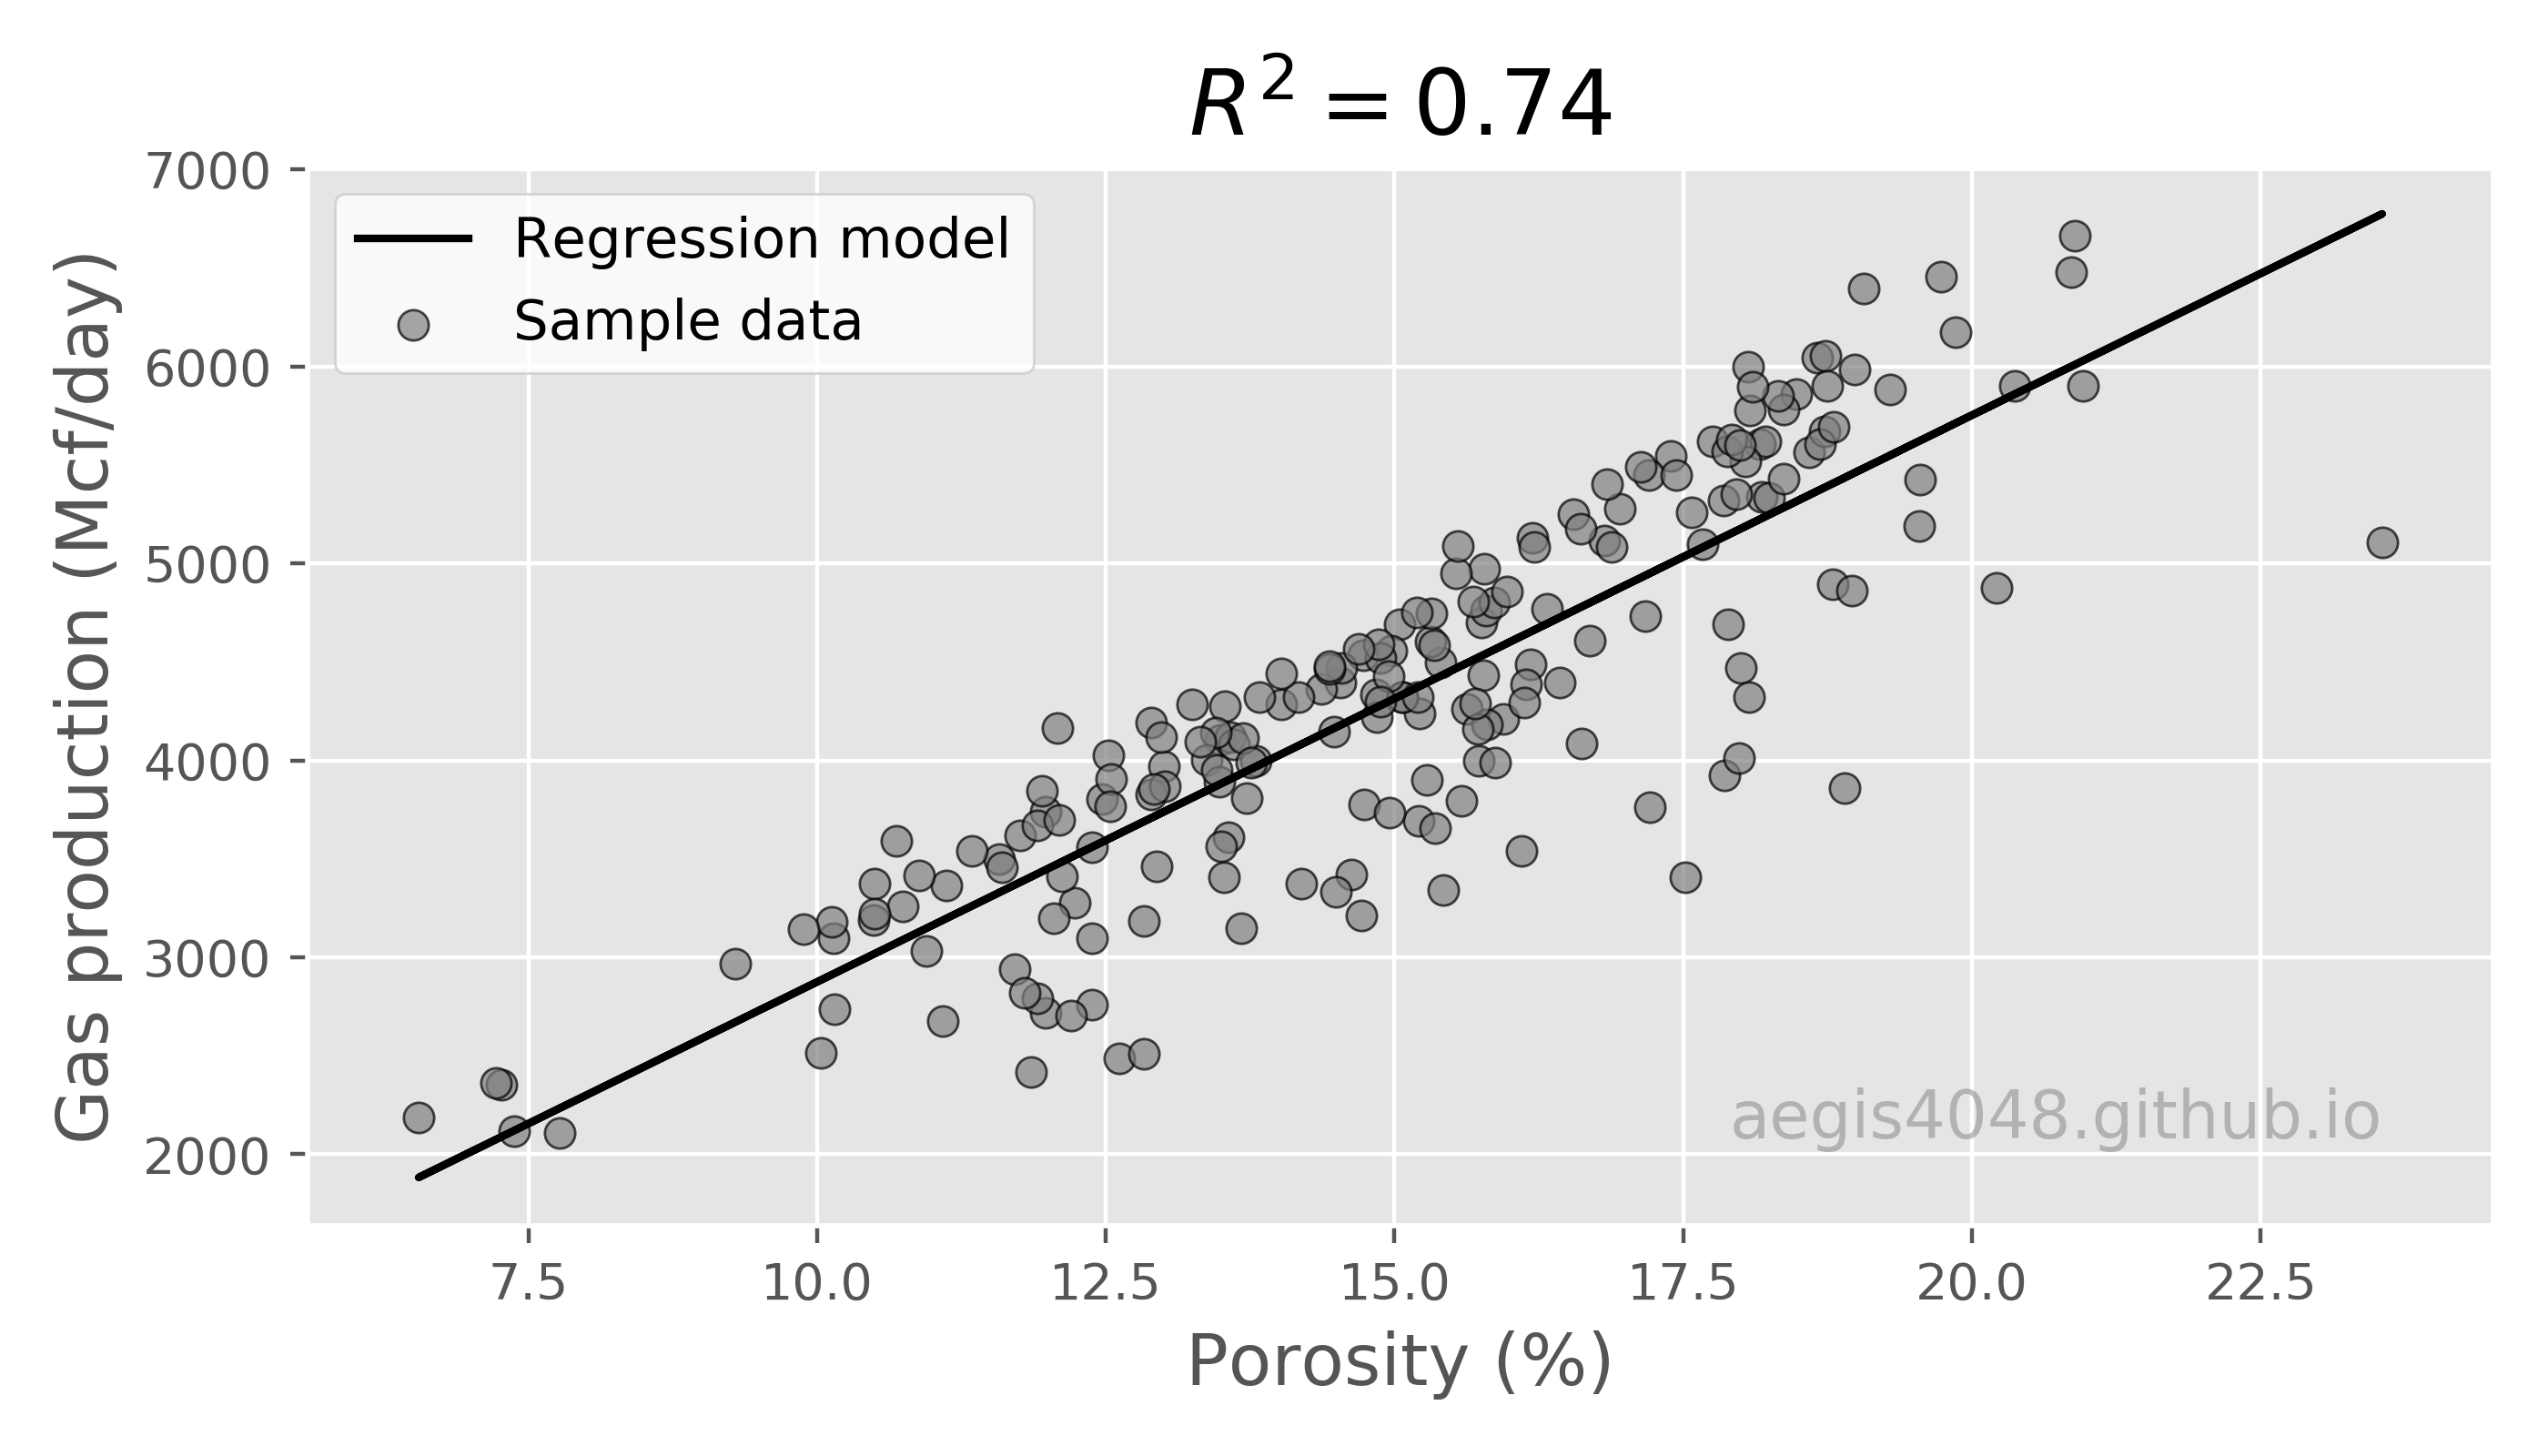
\includegraphics[width=\textwidth]{pictures/regresija.png}
    \caption{2D regresijski model, ki ga bomo seveda spremenili v avtorsko delo.}
    \label{fig:regresija}
\end{figure}

\section{Multipla regresijska analiza (logistična)}

Logistična regresija se uporablja, kadar je odvisna spremenljivka nominalna (ali binarna). Namesto linearne funkcije se uporablja logistična funkcija, ki omogoča napovedovanje kategorije odvisne spremenljivke.

Logistični model je podan kot:
\[\text{logit}(p) = \log\left(\frac{p}{1-p}\right) = \beta_0 + \beta_1 X_1 + \ldots + \beta_k X_k,\]
kjer je $p$ verjetnost, da se odvisna spremenljivka pojavi v določeni kategoriji.

\paragraph{Izračun koeficientov $\beta_i$}
Regresijski koeficienti $\beta_i$ se izračunajo z metodo največjega verjetja (Maximum Likelihood Estimation, MLE), ki išče koeficiente, ki maksimizirajo verjetnost opazovanih podatkov glede na model.

\paragraph{Interpretacija koeficientov $\beta_i$}
Koeficient $\beta_i$ predstavlja spremembo v logit(p) (logaritmu verjetnostnega razmerja) za enoto spremembe v $X_i$. Eksponentiranje koeficientov daje t.i. \emph{odds ratio} (razmerje verjetnosti):
\[\text{OR} = e^{\beta_i}\]
Odnos razmerja verjetnosti razlaga, kako se verjetnost pojavitve dogodka spremeni z enoto spremembe v $X_i$. Če je $\text{OR} > 1$, se verjetnost dogodka poveča, če je $\text{OR} < 1$, se verjetnost zmanjša.

\paragraph{Pseudo-$R^2$}
Za oceno kakovosti prileganja modela se v logistični regresiji pogosto uporablja t.i. pseudo-$R^2$. Ena izmed pogosto uporabljenih formul je McFaddenov pseudo-$R^2$:
\[R^2_{\text{McFadden}} = 1 - \frac{\log L_{\text{model}}}{\log L_{\text{null}}}\]
kjer je:
\begin{itemize}
    \item $\log L_{\text{model}}$ logaritmična verjetnost ustreznosti modela,
    \item $\log L_{\text{null}}$ logaritmična verjetnost modela brez neodvisnih spremenljivk (samo z interceptom).
\end{itemize}

McFaddenov pseudo-$R^2$ se giblje med 0 in 1, pri čemer višje vrednosti nakazujejo boljše prileganje modela.

\paragraph{Predpostavke logistične regresije}
\begin{itemize}
    \item \textbf{Neodvisnost opazovanj}: Vsako opazovanje mora biti neodvisno od drugih.
    \item \textbf{Neprekinjenost neodvisnih spremenljivk}: Neodvisne spremenljivke morajo biti kontinuirane ali binarne.
    \item \textbf{Linearnost logit transformacije}: Obstajati mora linearna povezava med logit(p) in neodvisnimi spremenljivkami.
\end{itemize}

\section{Razvrščanje v skupine (clustering)}

Razvrščanje v skupine ali clustering je metoda za razdelitev podatkov v več homogenih skupin na podlagi podobnosti med posameznimi podatkovnimi točkami. Najpogostejše metode vključujejo \textit{k-means}, \textit{hierarhično razvrščanje} in \textit{DBSCAN}.

\begin{figure}[h]
    \centering
    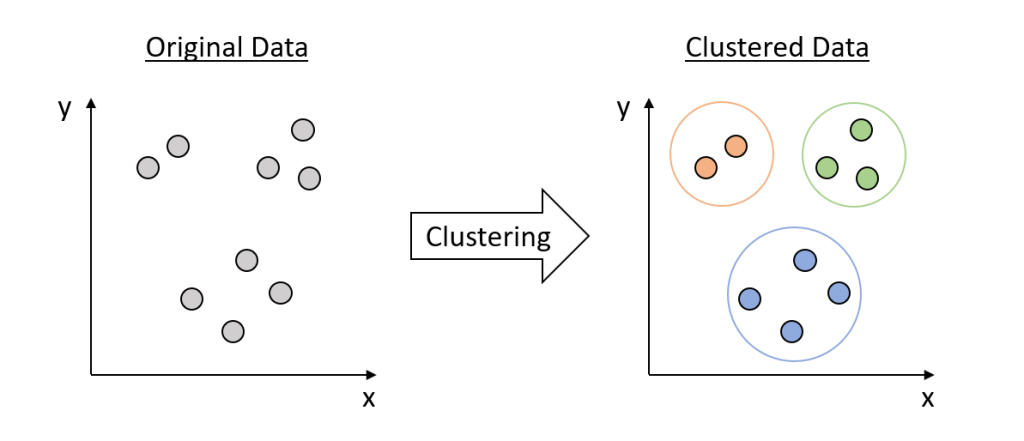
\includegraphics[width=\textwidth]{pictures/clustering.png}
    \caption{clustering, ki ga bomo seveda spremenili v avtorsko delo.}
    \label{fig:clustering}
\end{figure}


\paragraph{K-means clustering}
\textit{K-means} je ena najpogosteje uporabljenih metod za razvrščanje v skupine. Cilj algoritma je razdeliti podatke na $k$ skupin tako, da se minimizira vsota kvadratov odstopanj podatkovnih točk od njihovega pripadajočega centroida (povprečne vrednosti v skupini). Algoritem iterativno prilagaja centroidi do konvergence:
\[\text{min} \sum_{i=1}^{k} \sum_{x \in C_i} \| x - \mu_i \|^2,\]
kjer je $C_i$ skupina in $\mu_i$ centroid skupine $i$.

\section{Metode zmanjšanja dimenzionalnosti podatkov}

\textbf{Analiza glavnih komponent (PCA)}:
PCA je tehnika za zmanjšanje dimenzionalnosti podatkov, ki pretvori več povezanih spremenljivk v manj nepovezanih komponent. To omogoča lažjo vizualizacijo in analizo podatkov.

\textbf{Faktorska analiza}:
Faktorska analiza identificira latentne spremenljivke ali faktorje, ki pojasnjujejo vzorce korelacij med opazovanimi spremenljivkami. Model faktorske analize predpostavlja, da vsako opazovano spremenljivko $X_i$ lahko izrazimo kot linearno kombinacijo faktorjev $F_j$ in napake $\epsilon_i$:
\[X_i = \lambda_{i1} F_1 + \lambda_{i2} F_2 + \ldots + \lambda_{im} F_m + \epsilon_i,\]
kjer so $\lambda_{ij}$ faktorski uteži, ki kažejo na vpliv faktorja $F_j$ na spremenljivko $X_i$. Faktorska analiza se uporablja za zmanjšanje števila spremenljivk, hkrati pa ohranja interpretabilne latentne strukture.

\begin{figure}[h]
    \centering
    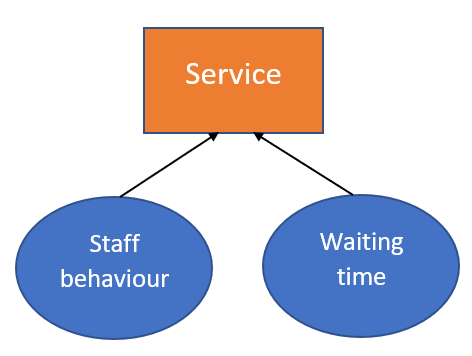
\includegraphics[width=0.5 \textwidth]{pictures/faktorska_analiza.png}
    \caption{faktorska analiza.}
    \label{fig:faktorska}
\end{figure}

\section{Analiza zanesljivosti}

\textbf{Cronbachov $\alpha$ koeficient}:
Cronbachov $\alpha$ koeficient je mera za notranjo konsistenco (zanesljivost) skale ali vprašalnika. Visoka vrednost $\alpha$ (bližje 1) nakazuje na visoko zanesljivost skale.

\subsection*{Formula za izračun Cronbachovega $\alpha$ koeficienta}

Cronbachov $\alpha$ se izračuna s pomočjo naslednje formule:

\[\alpha = \frac{k}{k - 1} \left(1 - \frac{\sum_{i=1}^{k} \sigma^2_{i}}{\sigma^2_{\text{skupaj}}}\right),\]

kjer:
\begin{itemize}
    \item $k$ je število postavk (vprašanj) v lestvici,
    \item $\sigma^2_{i}$ je varianca posamezne postavke,
    \item $\sigma^2_{\text{skupaj}}$ je varianca celotne lestvice (skupne ocene).
\end{itemize}

\subsection*{Interpretacija Cronbachovega $\alpha$}

\begin{itemize}
    \item $\alpha \geq 0.9$: Odlična (zelo visoka) zanesljivost
    \item $0.8 \leq \alpha < 0.9$: Dobra zanesljivost
    \item $0.7 \leq \alpha < 0.8$: Sprejemljiva zanesljivost
    \item $0.6 \leq \alpha < 0.7$: Vprašljiva zanesljivost
    \item $0.5 \leq \alpha < 0.6$: Slaba zanesljivost
    \item $\alpha < 0.5$: Nesprejemljiva zanesljivost
\end{itemize}

\subsection*{Pomembne točke}

\begin{itemize}
    \item \textbf{Uporaba Cronbachovega $\alpha$}: Najpogosteje se uporablja v psihometriji, pri preučevanju zanesljivosti vprašalnikov in testov. Pomembno je, da je lestvica homogena, kar pomeni, da vse postavke merijo en sam koncept.
    \item \textbf{Omejitve Cronbachovega $\alpha$}: Čeprav je $\alpha$ priljubljena mera, ni popolna. Visoka vrednost $\alpha$ ne pomeni nujno, da lestvica meri tisto, kar namerava meriti (validnost). Poleg tega lahko visoka vrednost $\alpha$ nastane tudi zaradi velikega števila postavk, ne pa nujno zaradi dejanske notranje konsistence.
    \item \textbf{Alternativne mere}: V nekaterih primerih se uporabljajo tudi druge mere zanesljivosti, kot je McDonaldov $\omega$, ki lahko poda natančnejšo sliko zanesljivosti v primerih, ko so postavke lestvice med seboj različno povezane.
\end{itemize}

\section{Druge multivariantne metode}

\paragraph{Kanonična korelacijska analiza:}
Kanonična korelacijska analiza je metoda za preučevanje povezave med dvema sklopoma spremenljivk. Omogoča določitev linearnih kombinacij spremenljivk iz obeh sklopov, ki so medsebojno najbolj povezane.

\paragraph{Diskriminantna analiza:}
Diskriminantna analiza je tehnika za razvrščanje opazovanj v predhodno določene skupine na podlagi neodvisnih spremenljivk. Uporablja se za napovedovanje kategorijske odvisne spremenljivke.

\paragraph{Strukturni modeli:}
Strukturni modeli so kompleksni statistični modeli, ki omogočajo preučevanje vzročnih odnosov med več spremenljivkami. Združujejo elemente regresijske analize, faktorske analize in poti.

\begin{Vaje}{1}
    V datoteki ... združi stolpce ... v eno spremenljivko ... in določi notranjo konsistentnost vprašalnika.
\end{Vaje}
